% !BIB TS-program = biber

\RequirePackage[l2tabu,orthodox]{nag}
\newcommand\todo[1]{\textcolor{red}{#1}}
% TODO: decide if one-sided/two-sided
%\documentclass[headsepline,footsepline,footinclude=false,fontsize=11pt,paper=a4,listof=totoc,bibliography=totoc,BCOR=12mm,DIV=12]{scrbook} % two-sided
\documentclass[headsepline,footsepline,footinclude=false,oneside,fontsize=11pt,paper=a4,listof=totoc,bibliography=totoc]{scrbook} % one-sided
\usepackage{amsmath}
\usepackage{tikz}
\usepackage{pgfplots}
\usepackage{pgfplotstable}
\pgfplotsset{compat=1.18}
\usetikzlibrary{arrows.meta, positioning,calc,patterns}
\usepackage{listings}
\usepackage{xcolor}
\usepackage{ wasysym }
\usepackage{hyperref}
\usepackage{subcaption}
\usepackage{algorithm}
\usepackage{algpseudocode}
\algrenewcommand\algorithmicfunction{\textbf{def}}
\algrenewcommand\algorithmicfor{\textbf{for}}
\algrenewcommand\algorithmicif{\textbf{if}}
\algrenewcommand\algorithmicdo{:}
\algrenewcommand\algorithmicthen{:}
\algtext*{EndFunction}
\algtext*{EndFor}
\algtext*{EndIf}

\newcommand\regpressure[1]{\textcolor{red}{\lightning #1}}
\newcommand{\bigO}{\mathcal{O}}

\definecolor{tumblue}{RGB}{0,101,189}
\definecolor{dkgreen}{rgb}{0,0.6,0}
\definecolor{mauve}{rgb}{0.58,0,0.82}

\definecolor{tumsec1}{RGB}{0,82,147}
\definecolor{tumsec2}{RGB}{0,51,89}
\definecolor{tumbeige}{RGB}{218,215,203}
\definecolor{tumorange}{RGB}{227,114,34}
\definecolor{tumgreen}{RGB}{162,173,0}
\definecolor{tumlblue}{RGB}{152,198,234}
\definecolor{tummidblue}{RGB}{100,160,200}

\definecolor{TLlightblue}{RGB}{119,170,221}
\definecolor{TLlightcyan}{RGB}{153,221,255}
\definecolor{TLmint}{RGB}{68,187,153}
\definecolor{TLpear}{RGB}{187,204,51}
\definecolor{TLolive}{RGB}{170,170,0}
\definecolor{TLlightyellow}{RGB}{238,221,136}
\definecolor{TLorange}{RGB}{238,136,102}
\definecolor{TLpink}{RGB}{255,170,187}
\definecolor{TLpalegray}{RGB}{221,221,221}
\definecolor{Fuchsia}{RGB}{140,54,140}
\definecolor{TBblue}{RGB}{68,119,170}
\definecolor{TBcyan}{RGB}{102,204,238}
\definecolor{TBgreen}{RGB}{34,136,51}
\definecolor{TByellow}{RGB}{204,187,68}
\definecolor{TBred}{RGB}{238,102,119}
\definecolor{TBpurple}{RGB}{170,51,119}
\definecolor{TBgrey}{RGB}{187,187,187}


\lstset{
  basicstyle=\footnotesize\ttfamily,
  columns=fullflexible,%
  keywordstyle=\bfseries\color{blue},%
  commentstyle=\color{dkgreen},%
  stringstyle=\color{mauve},%
}
\lstdefinestyle{asm}{
  basicstyle=\ttfamily\small,
  columns=fullflexible,
  keepspaces=true,
  frame=single,
  showstringspaces=false
}


% TODO: change thesis information
\newcommand*{\getUniversity}{Technische Universität München}
\newcommand*{\getFaculty}{Informatics}
\newcommand*{\getDegree}{Informatics}
\newcommand*{\getSchool}{Computation, Information and Technology}
\newcommand*{\getTitle}{Improving Register Allocation in a Fast Compiler}
\newcommand*{\getTitleGer}{Verbesserung der Registerallokation in einem schnellen Compiler}
\newcommand*{\getAuthor}{Thomas Saller}
\newcommand*{\getDoctype}{Master's Thesis}
\newcommand*{\getSupervisor}{Prof. Dr. Thomas Neumann}
\newcommand*{\getAdvisor}{Dr. Alexis Engelke}
\newcommand*{\getKeywords}{keyword;another keyword;one more}
\newcommand*{\getSubmissionDate}{08.04.2026}
\newcommand*{\getSubmissionLocation}{Munich}


% TODO: change citation style in settings
\input{settings}

\begin{document}



% Set page numbering to avoid "destination with the same identifier has been already used" warning for cover page.
% (see https://en.wikibooks.org/wiki/LaTeX/Hyperlinks#Problems_with_Links_and_Pages).
\pagenumbering{alph}
\input{pages/cover}

\frontmatter{}

\input{pages/title}
\input{pages/disclaimer}
\addcontentsline{toc}{chapter}{Acknowledgments}
\thispagestyle{empty}

\vspace*{20mm}

\begin{center}
    {\usekomafont{sectioning}\usekomafont{section} Acknowledgments}
\end{center}

\vspace{10mm}

%TODO: Acknowledgments
I would like to thank Alexis Engelke for the opportunity to write this thesis, as well as for his guidance and support throughout the process, without which this work would not have been possible. I also thank Tobias Schwartz for his time, support and guidance. 

Finally, I would like to thank the friends with whom I got to share my time at TUM, as well as my family whose support and encouragement was crucial for me to get to this point.

\cleardoublepage{}

\chapter{\abstractname}
Fast compilation is crucial in contexts where code generation occurs at runtime, such as query compilers in modern database systems or runtimes for modern programming languages. However, the quality of initially generated code is often markedly suboptimal, prompting many systems to adopt multi-tiered compilation strategies.

Recently, TPDE has shown that compilation speed of LLVM unoptimized back-end can be improved substantially while keeping a similar runtime. 
However, because TPDE further reduces compilation time at the unoptimized level, it also widens the compile-time gap to the next optimization level, \texttt{-O1}, to two orders of magnitude.

In this work, we present a novel register allocation approach built on top of TPDE that enables improved code generation while preserving a fast compilation time. By combining two analysis passes with a repair mechanism applied during code generation, our approach optimizes spill placement and resolves instruction constraints.

On SPECint 2017 we achieve a 24\% runtime improvement over the LLVM -O0 back-end, while maintaining a 4x faster compile time on optimized LLVM IR. Although, this also results in a 5x compile time slowdown compared to the original TPDE. Our results demonstrate the potential for a faster, lightly optimizing compiler back end; however, several design and implementation issues limit the performance of our approach.

\microtypesetup{protrusion=false}
\tableofcontents{}
\microtypesetup{protrusion=true}

\mainmatter{}

% !TeX root = ../main.tex
% Add the above to each chapter to make compiling the PDF easier in some editors.
% Read the CSV files

\chapter{Introduction}\label{chapter:introduction}

Just-in-time (JIT) compilation is a widely used technique for improving performance for applications, where the combined speed of compilation and execution is critical. Such
applications include dynamic runtimes such as the Java Virtual Machine~\cite{jvm} as well as
the acceleration of database queries~\cite{sql-jit}. 

Since compile time directly contributes to end-to-end latency, fast machine code generation is especially important for JIT compilation. Recently, TPDE~\cite{tpde} has shown that the compilation speed of the LLVM~\cite{LLVM} unoptimized back-end can be improved substantially, while keeping a similar runtime performance. 

Since JIT systems inherently involve a trade-off between compilation and runtime, many
systems employ multi-stage approaches, with the first stage serving as the baseline and subsequent stages being progressively optimized~\cite{tpde}.
However, when using LLVM, the difference in compilation time between TPDE and LLVM's optimized backend (\texttt{-O1}) is two orders of magnitude, leaving a significant gap for programs that could benefit from better code generation, but for which the substantial increase in compilation time cannot be justified.

To address this gap, we propose a novel register allocation approach built on top of TPDE that enables improved code generation while maintaining relatively fast compilation times. Our approach consists of two analysis passes: a liveness analysis, which additionally computes next-use information, and a spill analysis pass that determines which values to spill and optimizes spill locations to reduce spill overhead in loops. During code generation, we introduce a repair mechanism for handling instruction constraints, enabling more efficient code generation for constrained operations such as integer division on \texttt{x86-64}.

On SPECint 2017, we achieve a 24\% runtime improvement over the LLVM-O0 backend,
while the compilation time for optimized LLVM-IR remains three times faster. However,
this also results in a 5x increase in compilation time compared to TPDE. Nevertheless, our work achieves a
new Pareto optimum for the compilation of optimized IR, as it is significantly faster than LLVM-O1 in terms of compilation time,
while simultaneously offering a runtime improvement over both
TPDE and LLVM-O0.
\newpage
The key contributions of our work include:

\begin{itemize}
    \item A lifetime analysis that generates next-use information in the same pass
    \item A spill analysis that identifies values to spill without relying on knowledge of the instruction semantics, or requiring modification to the IR.
    \item A simplified repairing mechanism to handle instruction constraints during code generation, without rolling back code generation.
\end{itemize}

The remainder of this work is structured as follows: In \autoref{ch:background} we provide background on register allocation and TPDE, as well as the constraints arising from the framework’s design. In \autoref{chapter:approach} we present our approach. In \autoref{chapter:related_work} we discuss related work in register allocation, and how it relates to our approach. Next we evaluate our approach compared to TPDE, LLVM-O0 and LLVM-O1 in \autoref{chapter:evaluation}. Finally, we summarize our results and discuss future work in \autoref{chapter:conclusion}.
% !TeX root = ../main.tex
\chapter{Background}
\label{ch:background}
In this chapter, we will introduce the basic concepts of register allocation and the particular importance of the SSA form. We then brievely describe the TPDE backend framework and the resulting challenges building register allocation on top of it.

\section{Register Allocation on non-SSA programs}
\label{sec:regalloc-non-ssa}

Register Allocation is the process of assigning values from a program to a limited number of $k$ physical registers. This process is commonly modeled as finding the Graph Coloring of an Interference graph corresponding to the program.

The nodes in an intereference graph correspond to the values in a program, and edges between them indicate that the connected values interfere with eachother and therefore cannot be in the same register. This nicely corresponds to Graph coloring where connected nodes may not be assigned the same color.

Therefore a valid coloring with at most $k$ colors would be a valid register allocation for the corresponding program on an perfectly regular archtiecture with at least $k$ registers.

In practice, using such an approach directely is unfeasible as GC is NP-complete in the number of values~\cite{graph-coloring-np-complete}, and any arbitrary IG can be used to construct a program having the same IG~\cite{chaitin1981}. 
In addition, deciding how many registers a program requires and deciding wether $k$ registers are sufficient are also NP-complete~\cite{hack-thesis}.

Practical RA need to rely on heuristics at all steps, to find a allocation in a reasonable time. We will illustrate this with the seminal work by Chaitin~\cite{chaitin1981} on the subject. Note that we will assume a theoretical regular architecture for now. We will address archtectural constraints and their associated complications later.

\subsection{Chaitlin Style Graph Coloring Register Allocation}

\begin{figure}
\centering
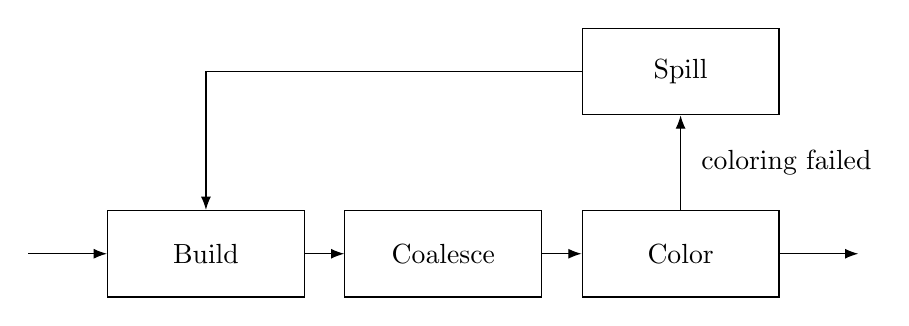
\begin{tikzpicture}[
    >=Latex,
    box/.style={
        draw,
        minimum width=2.5cm,
        minimum height=1.1cm,
        align=center
    }
]

% Nodes
\node[box] (build) {Build};
\node[box, right=0.5cm of build] (coalesce) {Coalesce};
\node[box, right=0.5cm of coalesce] (color) {Color};
\node[box, above=1.2cm of color] (spill) {Spill};

% Main horizontal flow
\draw[->] ($(build.west)+(-1.0,0)$) -- (build.west);
\draw[->] (build.east) -- (coalesce.west);
\draw[->] (coalesce.east) -- (color.west);
\draw[->] (color.east) -- ++(1.0,0);

% Upward failure edge
\draw[->] (color.north) -- node[right=4pt] {coloring failed} (spill.south);

% Back edge from Spill to Build
\draw[->] (spill.west) -| (build.north);

\end{tikzpicture}
\caption{Simplified overview of the steps in a graph coloring allocator}
\label{fig:graph-coloring-steps}
\end{figure}

First the Interference Graph itself has to be constructed. This is done by scanning the program and adding edges between values that are live at the same time. 

Next, a coalescing heuristic is applied such that the nodes stemming from copy instructions are merged into a single node. Notice that this step might increase the number of colors required for the new graph since, the merged nodes may have more edges than previously. 

Finally, the main coloring step begins. First all nodes with fewer than $k$ neighbors are removed from the graph and placed into a stack. If the graph is now empty, we move on to the next step. Otherwise, we select a remaining node for spilling and rebuild the IG for the new program after inserting spill code. This process is repeated until the graph is empty.

Now all nodes are on the coloring stack, where we reinsert them into the graph and assign them a color. This will always be possible since they must have fewer than $k$ neighbors. This produces a valid coloring of the final program.

While this approach produces good results in practice, building the Inference Graph is an expensive operation and the iterative nature of the algorithm make it unattractive for use in a JIT compiler~\cite{Cooper06}. 

While there have been countless improvements to the original algorithm, the basic iterative structure remains the same, prompting different approaches to the problem.

\subsection{Other Approaches}

One alternate approach is to formulate Register Allocation as an Integer Linear Programming problem. While this can produce optimal results it is also NP-complete and the worst case runtimes of several minutes makes them unattractive for JIT compilers\cite{ilp-regalloc}.

The other common approach is to use a linear scan allocator~\cite{linear-scan-og}. This approach avoids the expensive IG datastructure in favor of using a total ordering of all program instructions. This ordering is used to determine the single live range of each value, for example starting at instruction $i$ and ending at instruction $j$ ($[i,j]$). The live ranges are then assigned to registers in the order of their interval start. 

Once the algorithm runs out of registers, it spills a value, splitting its live range into two parts. The spilled value is typically chosen based upon the furthest live range end.

This approach is simple and non-iterative and therefore attractive for use in a JIT compiler. However, due to the simplified liveness information, the resulting allocation quality is comparatively worse. Especially around control flow such as loops and branches with differing register pressure. Although there have been multiple improvements from the original algorithm, the resulting allocation quality is considered worse than that of graph coloring~\cite{wimmer-06-linear-scan}.

\section{Register Allocation on SSA programs}


% TODO: add more chapters here
% !TeX root = ../main.tex
% Add the above to each chapter to make compiling the PDF easier in some editors.

\chapter{Approach}\label{chapter:approach}

\section{Fast Liveness}
A non iteraite liveness analysis on strict SSA.

\section{combining liveness sets and next-use distance}

\section{Spilling with next-use distance}
\begin{itemize}
    \item Irreducable control flow
    \item Spill on definition
\end{itemize}

\section{Register Allocation with Repairing}
\begin{itemize}
    \item Multi- part challenges
\end{itemize}

\section{VerificationIR (kind of useless)}
% !TeX root = ../main.tex
% Add the above to each chapter to make compiling the PDF easier in some editors.

\chapter{Related Work}\label{chapter:related_work}
 
As explained previously in \autoref{sec:tpde}, our work has access to less information than is typical. Therefore,  all approaches discussed in this chapter would require significant adaptations to be applicable in TPDE.

To the best of our knowledge, there is no existing work, intended for use without knowledge of the instruction selection and the instruction constraints.
% todo impact of ssa form?



% linear scan dann in Related work und puzzle solving zeugs
\section{Graph Coloring Register Allocation}


As previously described, graph coloring of interference graphs is equivalent to register allocation~\autocite{chaitin1981}. 
In general this is a NP-hard problem~\autocite{chaitin1981}. For graphs that cannot be colored with k colors, graph coloring algorithms must also iterate between coloring, spilling and coalescing. Each spill step requiring an expensive rebuild of the interference graph~\autocite{Cooper06}. This makes traditional graph coloring register allocation too slow for just in time compilation~\autocite{Cooper06}. 

Compared to GC approaches our work involves only 2 preprocessing passes, including lifetime  analysis, and does not require any iterative algorithms, which allows for a more predictable runtime. 

The cost of rebuilding the interference graph after every spilling step can be avoided by approximating the resulting interference graph using additional metadata~\autocite{Cooper06}. This sacrifices a small amount of code quality for a significant speedup, which makes it more suitable for just in time compilation. However, the IG remains expensive to build even once and the algorithm remains iterative, and therefore remains less suitable for our use case.

We will consider such SSA-based algorithms such as ours separately as they have different compilation speed properties, even though they are fundamentally based on graph coloring.

\section{Linear Scan Register Allocation}
Linear scan allocators perform a single scan of the program to find live ranges, which are then mapped to registers or memory~\cite{linear-scan-og}.
Compared to graph coloring, linear scan requires only one pass over the program and no costly construction of an interference graph. However, their code quality is generally worse than graph coloring~\cite{hack-thesis}.
We use a similar approach with one final code generation pass, although we use a precise liveness analysis. Additionally, we have a separate spilling pass, which is crucial for optimizing spill locations around loops.

While some limitations of the original algorithm, such as the lack of lifetime holes for control flow, have been addressed~\cite{Wimmer2010}. 
Linear scan allocators fundamentally use a non-optimal approach involving increasingly elaborate heuristics or post-processing passes to improve code quality~\cite{Wimmer2010}.

Similar to improvements by Wimmer and Franz~\cite{Wimmer2010}, our approach precomputes a set of spilled variables, allowing for better spill locations compared to spilling once the algorithm runs out of registers. As opposed to the later modifications to linear scan, we cannot change allocated code afterwards, which limits the applicability of the proposed improvements. In particular,  it would not be possible to move spills in our work.
Due to this limitation, our preprocessing steps are responsible for finding good spill locations. 

Since our code generation step remains as a single pass, our approach could be considered a modified variant of linear scan with additional preprocessing stages.

\section{Trace Register Allocation}
In particular, for JIT compilers, trace allocation can be used to assign registers on chosen segments, so-called traces, that don't contain control flow~\cite{trace-ra}. This allows for a fast algorithm that can use different allocation strategies based on the trace properties. 
However, choosing good traces is non-trivial without runtime profiling information, and the resulting code quality is highly dependent on the trace selection~\cite{trace-ra}.

As TPDE~\cite{tpde} does not use have access to runtime profiling information, this approach is not suitable for our use case. Our approach allocates across control flow,  without runtime information, based on the assumption that loops will be executed multiple times.

\section{SSA Register Allocation}

These strategies utilize the favorable properties of SSA form to avoid the runtime costs of traditional graph coloring approaches. Although adapting these results for real architectures with constrained instructions and no swap instructions requires live range splitting and additional modifications to the IR~\cite{hack-thesis}.
Such modifications would be difficult to integrate into TPDE, as it cannot modify the underlying IR, in addition TPDE lacks the information about constraints before code generation.

Instead of modifying the program, as was previously required, an alternative approach introduces the notion of repairing if an irregularity is encountered~\cite{treescan}. 
By allowing deviations in the register set at such points, they propose a simpler algorithm that falls back on graph coloring in situations where a repair using parallel moves is not possible.
We adopt a similar approach to Colombet et al.~\cite{treescan} by introducing preferred registers and repairing around constraints, however we do not use repairing across all operands of an instruction, thereby limiting our code quality for highly constrained instructions. For calls, our approach is equivalent, although we cannot fall back to a graph coloring approach should the repairing fail.
% !TeX root = ../main.tex
% Add the above to each chapter to make compiling the PDF easier in some editors.

\chapter{Evaluation}\label{chapter:evaluation}
\section{Correctness}
We verify the correctness of our implementation by using the LLVM test suite and by running the SPEC CPU2017 integer benchmarks. Except for some LLVM test cases that contain unsupported instructions, all tests pass sucessfully on AArch64 and x86-64. Which we assume is a good proxy for the correctness of our implementation.

\section{Performance}

\subsection{Setup}
We evaluate the performance of our implementation by measuring the back-end
compile-time and the run-time performance of LLVM-IR generated by Clang. We use code produced
with -O1, where variables are in SSA form. We
compare our implementation against the original version of TPDE and against both the LLVM-O0 and LLVM-O1 back-end, the former two focusing on compile-time and the latter being a optimizing back-end. 
As benchmark programs, we use the SPEC CPU2017 integer benchmarks on x86-64 and AArch64.
Our x86-64 machine is an Amd Ryzen 5 5600X with 32 GiB of RAM running Linux \todo{version}; Our
AArch64 machine is an Apple M1 with 16 GiB of memory, using only the four performance cores,
running Asahi Linux \todo{version}. We use Clang/LLVM version 20.1.8.


% !TeX root = ../main.tex
% Add the above to each chapter to make compiling the PDF easier in some editors.


\chapter{Conclusion and Future Work}\label{chapter:conclusion}

In this thesis we presented a novel register allocation approach built on top of TPDE, allowing for better code generation, without requiring information on the specific instruction semantics, and maintaining the core single-pass code generation.

We introduced a lifetime and next-use analysis, as well as a spill analysis that approximates register pressure and optimizes spill locations around loops. During code generation, we introduced a repairing mechanism to preserve values across constrained instructions, by inserting moves.


On the SPECint 2017 benchmark, we achieved a 24\% runtime improvement over the LLVM \texttt{-O0} backend while maintaining a compile time that was three times faster on optimized LLVM IR. However, this also incurs a sixfold increase in compile time compared to TPDE. Despite the overall improvements, we observe no difference for certain benchmarks due to limitations in our approach when using optimized LLVM IR, which was not designed for use in code generation without further transformations.

Future work may address these limitations by implementing additional analyses, specifically around \texttt{getelementptr} instructions with constant offsets, which are a limiting factor for our approach. Storing such values as offsets from a base pointer would enable better code generation, especially for the worst-performing benchmarks. However, this would potentially require additional modifications to the base TPDE framework, which is intended to be IR-agnostic. 

Additionally, code quality could be improved by implementing a more elaborate repair mechanism that can handle shuffling multiple operands for a constrained instruction. Finally, a better heuristic could prevent spills for loops with low register pressure, as illustrated in \autoref{fig:asm}.

The compile-time overhead could be reduced by optimizing our implementation, particularly by minimizing the number of allocations caused by set and map operations.





\appendix{}

\microtypesetup{protrusion=false}

\addchap{Abbreviations}
\begin{acronym}
	\itemsep-.25\baselineskip
	\acro{SSA}[SSA]{Static Single Assignment}
	\acro{RA}{Register Allocation}
  \acro{GC}{Graph coloring}
  \acro{IR}{Intermediate representation}
  \acro{LICM}{Loop invariant code motion}
  \acro{CFG}{Control flow graph}
	% TODO: add acronyms
\end{acronym}

\listoffigures{}
\listoftables{}
\microtypesetup{protrusion=true}
\printbibliography{}

\end{document}
